\documentclass[french, a4paper, 10pt]{article}

\usepackage{babel}
\usepackage[T1]{fontenc}
\usepackage[utf8x]{inputenc}

\usepackage[top=2.5cm, bottom=2.5cm, left=2.5cm, right=2.5cm]{geometry}
\usepackage{url}
\usepackage{hyperref}
\usepackage{float}
\usepackage{nicefrac}

\usepackage{chemist}
\usepackage{siunitx}
\usepackage{amsmath}
\usepackage{cases}

\usepackage[numbered,framed]{matlab-prettifier}

\DeclareSIUnit\jour{j}
\sisetup{per-mode=fraction, fraction-function=\nicefrac}
\newcommand{\dotc}[2]{\dot{#1}_{\text{\chemform{#2}}}}

\usepackage{pgffor}
\usepackage{xifthen}
\usepackage{fancyhdr}
\usepackage{graphicx}
\newcommand{\hyperauthors}[2]{
	\textbf{Groupe #1} \\
	\foreach \i/\q in {#2}{
		\textsc{\q} \i \\
  	}
}
\newcommand{\hypertutors}[1]{
	\textbf{Tuteur(s) : } \\
	\foreach \i/\q in {#1}{
		\textsc{\q} \i \\
	}
}
\newcommand{\hypertitle}[7]{
	% #1 Title
	% #2 Cours 
	% #3 Numéro de groupe
	% #4 Membres du groupe, format : {prenom/nom, prenom/nom, ...}
	% #5 Tuteurs, même format que membres
	% #6 si existe -> toc
	% #7 Date
	\fancyhf{} %clear all headers and footers fields
	\fancyhead[R]{\thepage} %prints the page number on the right side of the header
	\fancyhead[L]{#1}


	\pagestyle{fancy}
	\thispagestyle{empty}
	\begin{titlepage}
		\begin{center}
			
\includegraphics[width=0.15\textwidth]{pictures/logo.JPG}~\\[1cm]
			\textsc{\LARGE Université Catholique de Louvain}\\[1.5cm]
			\textsc{\Large #2}\\[0.5cm]

			\rule{\linewidth}{0.5mm} \\[0.4cm]
			{ \huge \bfseries #1\\[0.4cm] }
			\rule{\linewidth}{0.5mm} \\[1.5cm]
			
			\begin{minipage}{0.4\textwidth}
				\begin{flushleft} \large
					\hyperauthors{#3}{#4}
				\end{flushleft}
			\end{minipage}
			\begin{minipage}{0.4\textwidth}
				\begin{flushright} \large
					\ifthenelse{\isempty{#5}}{}{\hypertutors{#5}}
				\end{flushright}
			\end{minipage}
			\ifthenelse{\isempty{#6}}{}{\tableofcontents}

			\vfill

			{\large #7}
		\end{center}
	\end{titlepage}

	\clearpage
	\pagenumbering{arabic}
	\newpage

	\thispagestyle{empty}
}


\begin{document}
\hypertitle{Thématique 2 : Gestion de la production}{LFSAB1503 Projet 3}{12.64}{Paul/Asselberghs, Brice/Bertin, Adrien/Couplet, Grégory/Creupelandt, Anthony/Gatin, Antoine/Gennart, Juline/Gillard, Pierre/Martin}{}{}{\today}

\tableofcontents

\newpage
\part{Introduction}
Ce document a pour but d'étudier les bilans de matière et d'énergie d'un procédé alternatif de production d'ammoniac. Nous avons calculé pour chaque unité du procédé les débits d'entrée et de sortie ainsi que l'énergie et les températures dans l'unité de reformage autotherme. À partir des calculs obtenus dans ce document, il nous sera possible de développer un outil de simulation permettant d'étudier l'influence de paramètres sur le fonctionnement du procédé. 
\begin{figure}[h]
	\centering
	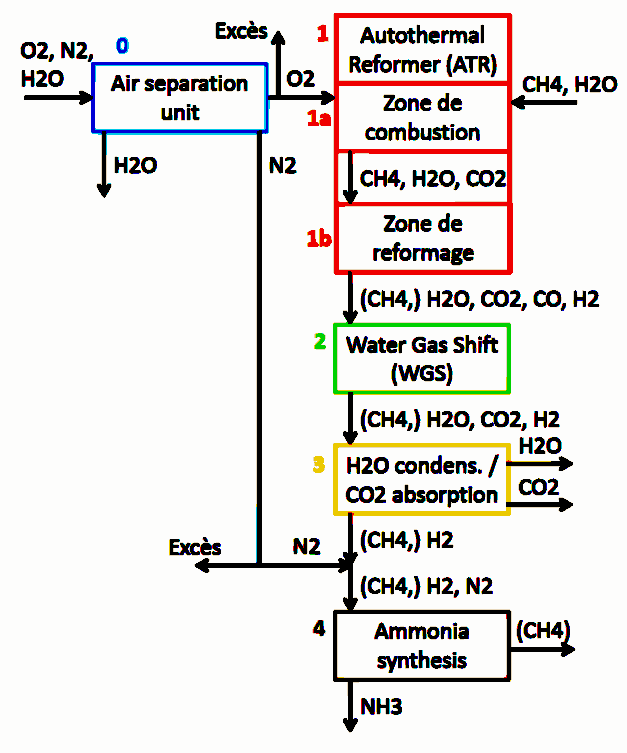
\includegraphics[width=0.5\textwidth]{pictures/procede.pdf}
	\caption{\label{fig:procede}Flow-sheet simplifié de la production d'ammoniac avec ATR}
\end{figure}

\section{Propriétés et hypothèses physico-chimique}
Avant de commencer les calculs, il est necéssaire de faire quelques hypothèses afin de les simplifier : 
\begin{enumerate}
	\item La réaction de combustion de l'ATR (voir partie suivante, équation \ref{eq:combustion}) est considérée complète. Il n'en ressort que du \chemform{CO_2} et de l'\chemform{H_2O}. Normalement, dans le cas d'une combustion incomplète, un manque d'\chemform{O_2} aurait permit la formation de \chemform{CO} qui aurait interferé avec la suite du procédé.
	\item La réaction dans l'unité Water Gas Shift est considérée complète (équation \ref{eq:wgs}. Il est à noter que la même réaction survient plus tôt dans la zone de reformage mais de manière incomplète (équation \ref{eq:reformage2}). 
	\item Dans l'unité de condensation et d'absorption nous émettons l'hypothèse que nous retirons uniquement et complètement le \chemform{H_2O} et \chemform{CO_2} du procédé.
	\item En dehors des unités opérationelles, les réactifs ne réagissent pas entre eux.
	\item La réaction de synthèse de l'ammoniac (équation \ref{eq:synthese}) est considérée comme complète.
	\item Les quelconques pertes d'énergie entre les unités opérationelles sont négligeables. 
	\item Les paramètres initiaux qui nous sont donnés sont considérés comme exacts, sans marge d'erreur.
	\item L'unité de séparation de l'air effectue une séparation complète.
\end{enumerate}
\begin{table}[H]
	\centering
	\begin{tabular}{lccp{6cm}}\hline
		\textbf{Paramètre} & \textbf{Valeur} & \textbf{Unité} & \textbf{Description} \\\hline
		$K_{\text{SMR}}$ & $10^{\left(\frac{-11650}{T}+13.076\right)}$ & - & Constante d'équilibre du reformage du méthane (\textbf{S}team \textbf{M}ethane \textbf{R}eforming). La température $T$ est en \si{K}.\\
		$K_{\text{WGS}}$ & $10^{\left(\frac{1910}{T}-1.764\right)}$ & - & Constante d'équilibre de la réaction du gaz à l'eau (\textbf{W}ater-\textbf{G}as \textbf{S}hift). La température $T$ est en \si{K}.\\
		$\Delta H^0_{\text{\chemform{CH4},comb},\SI{1200}{\kelvin}}$ & -803 & \si{\kilo\joule\per\mol} & Variation d'enthalpie de l'oxidation complète du méthane en \chemform{CO_2} et \chemform{H_2O} à \SI{1200}{\kelvin}. On peut considérer cette valeur constante pour les températures que nous atteindrons. \\
		$\Delta H^0_{\text{SMR},\SI{948}{\kelvin}}$ & 224.0 & \si{\kilo\joule\per\mol} & Variation d'enthalpie du reformage du méthane à \SI{948}{\kelvin}. On peut considérer cette valeur constante pour les températures que nous atteindrons. \\
		$\Delta H^0_{\text{WGS},\SI{948}{\kelvin}}$ & -37.3 & \si{\kilo\joule\per\mol} & Variation d'enthalpie de la réaction du gaz à l'eau à \SI{948}{\kelvin}. On peut considérer cette valeur constante pour les températures que nous atteindrons. \\
		$c_{p,g}$ & 2500 & \si{\joule\per\kilo\gram\per\kelvin} & Capacité thermique moyenne du mélange gazeux de l'ATR. On peut considérer cette valeur constante.\\\hline
	\end{tabular}
	\caption{\label{tab:proprietes}Propriétés physico-chimiques et hypothèses nécessaires pour les bilans de matière et d'énergies}
\end{table}


\newpage
\part{Bilan de matière}
Pour faciliter nos calculs nous considérons le symbole $\dot{n}$ comme étant le débit molaire avec comme unité le nombre de mol produit par seconde (\si{\mol\per\second}).
Nous commencerons par calculer pour toutes les étapes du procédé les bilans de matière. À base de ceux-ci nous déterminerons les débits de production d'ammoniac, d'alimentation d'air, ainsi que tous les débits intermédiares entres les unités opérationnelles.
Deuxièmement nous étudierons ce bilan avec des paramètres donnés. 

\section{Méthode de calcul des débits molaires}
Les débits molaires que nous utilisons dans nos calculs dépendent de l'unité dans laquelle ils sont calculés. Par exemple le $\dotc{n}{CH_4}$ de la zone de combustion n'est pas le même que celui de la zone de reformage. Au début de chaque unité nous reprenons les débits de l'unité précédente. Nous rappelons au lecteur que le symbole $\dot{n}_i$ correspond au débit molaire en entrée (avant réaction) et $\dot{n}_f$ au débit molaire en sortie (après réaction).
\subsection{ATR : zone de combustion}
Nous commencons par la zone de combustion où se produit une combustion du méthane dans le dioxygène :
\begin{chemeqn}
	CH_4 + 2O_2 \longrightarrow CO_2 + 2H_2O
	\label{eq:combustion}
\end{chemeqn}
\begin{table}[h]
	\centering\renewcommand{\arraystretch}{1.2}
	\begin{tabular}{l|ccccccc}
		& \chemform{CH_4} & + & \chemform{2O_2} & $\longrightarrow$ & \chemform{CO_2} & + & \chemform{2H_2O} \\\hline
		$\dot{n}_i$ & $\dotc{n}{CH_4}$ && $2\dotc{n}{O_2}$ && 0  && $\dotc{n}{H_2O}$  \\
		$\dot{n}_f$	& $\dotc{n}{CH_4}-\dotc{n}{O_2}$ && 0  && $\dotc{n}{O_2}$ && $\dotc{n}{H_2O}+2\dotc{n}{O_2}$ \\
	\end{tabular}
	\caption{\label{tab:combustion}Avancement de la combustion du méthane}
\end{table}

\subsection{ATR : Zone de reformage}
Nous passons ensuite au reformage à la vapeur du méthane (en anglais: \textit{steam methane reforming}, SMR). Cette étape est constituée de deux réactions incomplètes : 
\begin{enumerate}
	\item La réaction incomplète du méthane avec l'eau permettant de produire l'hydrogène nécessaire à la suite du procédé : 
		\begin{chemeqn}CH_4+H_2O \rightleftharpoons 3H_2 + CO\label{eq:reformage1}\end{chemeqn}
	\item La réaction incomplète du gaz à l'eau (WGS) due au monoxyde de carbone réagissant avec l'eau. Cette réaction produit elle aussi de l'hydrogène :
		\begin{chemeqn}CO + H_2O \rightleftharpoons H_2 + CO_2\label{eq:reformage2}\end{chemeqn}
\end{enumerate}
Les deux réactions se produisent simultanément, il est donc impossible de les considérer de manière individuelle.
\begin{table}[H]
	\centering\renewcommand{\arraystretch}{1.1}
	\begin{tabular}{l|ccccccc}
		& \chemform{CH_4} & + & \chemform{H_2O} & $\rightleftharpoons$ & \chemform{3H_2} & + & \chemform{CO} \\\hline 
		$\dot{n_0}$ & $\dotc{n}{CH_4}$ && $\dotc{n}{H_2O}$ && 0 && 0 \\
	   	$\dot{n_f}$ & $\dotc{n}{CH_4}-\xi$ && $\dotc{n}{H_2O}-\xi-\beta$ && $3\xi+\beta$ && $\xi-\beta$ \\	
	\end{tabular}
	\caption{\label{tab:reformage1}Avancement du premier équilibre chimique ($\xi$)}
\end{table}
\begin{table}[H]
	\centering\renewcommand{\arraystretch}{1.1}
	\begin{tabular}{l|ccccccc}
		& \chemform{CO} & + & \chemform{H_2O} & $\rightleftharpoons$ & \chemform{H_2} & + & \chemform{CO_2} \\\hline 
		$\dot{n_0}$ & 0 && $\dotc{n}{H_2O}$ && 0 && $\dotc{n}{CO_2}$ \\
	   	$\dot{n_f}$ & $\xi-\beta$ && $\dotc{n}{H_2O}-\xi-\beta$ && $3\xi+\beta$ && $\dotc{n}{CO_2}+\beta$ \\	
	\end{tabular}
	\caption{\label{tab:reformage2}Avancement du deuxième équilibre chimique ($\beta$)}
\end{table}
On déduit ensuite pour chaque équilibre l'expression de la constante d'équilibre :
\begin{align}
K_\text{SMR} &= \frac{(\xi-\beta)(3\xi+\beta)^3}{(\dotc{n}{H_2O}-\xi-\beta)(\dotc{n}{CH_4}-\beta)}\cdot\frac{p_t^2}{(\dotc{n}{CH_4}+\dotc{n}{H_2O}+\dotc{n}{CO_2}+2\xi)^2}\\
K_\text{WGS} &= \frac{(\dotc{n}{CO_2}+\beta)(3\xi+\beta)}{(\xi-\beta)(\dotc{n}{H_2O}-\xi-\beta)}
\end{align}
À partir des propriétés physico-chimiques (table \ref{tab:proprietes}) et de la température dans l'ATR donnée en paramètre nous pouvons déterminer les valeurss de $K_\text{SMR}$ et $K_{WGS}$ : 
\begin{align}
	K_\text{SMR} &= 10^{\left(\frac{-11650}{T}+13.076\right)} \\
	K_\text{WGS} &= 10^{\left(\frac{1910}{T}-1.764\right)} 
\end{align}
Nous avons alors un système de deux équations à deux inconnues ($\xi$ et $\beta$) 
\begin{equation}
	\left\{
	\begin{aligned}
		10^{\left(\frac{-11650}{T}+13.076\right)} &= \frac{(\xi-\beta)(3\xi+\beta)^3}{(\dotc{n}{H_2O}-\xi-\beta)(\dotc{n}{CH_4}-\beta)}\cdot\frac{p_t^2}{(\dotc{n}{CH_4}+\dotc{n}{H_2O}+\dotc{n}{CO_2}+2\xi)^2}\\
		10^{\left(\frac{1910}{T}-1.764\right)}    &= \frac{(\dotc{n}{CO_2}+\beta)(3\xi+\beta)}{(\xi-\beta)(\dotc{n}{H_2O}-\xi-\beta)}
	\end{aligned}
	\right.
\end{equation}
que nous résolvons à l'aide du logiciel Matlab\textsuperscript{\textregistered} avec la fonction suivante :
\lstinputlisting[style=Matlab-editor, basicstyle=\scriptsize\ttfamily, tabsize=4, caption=Code Matlab\textsuperscript{\textregistered} pour résoudre le système\label{lst:matlab}]{ressources/reformage.m}
Au final, nous obtenons à la sortie de la zone de reformage les débits suivants :
\begin{table}[H]
	\centering\renewcommand{\arraystretch}{1.1}
	\begin{tabular}{l|ccccc}
		& \chemform{CH_4} & \chemform{H_2O} & \chemform{CO_2} & \chemform{CO} & \chemform{H_2}\\\hline
		$\dot{n_0}$ & $\dotc{n}{CH_4}$ & $\dotc{n}{H_2O}$ & $\dotc{n}{CO_2}$ & 0 & 0 \\
		$\dot{n_f}$ & $\dotc{n}{CH_4}-\xi$ & $\dotc{n}{H_2O}-\xi-\beta$ & $\dotc{n}{CO_2}+\beta$ & $\xi-\beta$ & $3\xi+\beta$
	\end{tabular}
	\caption{\label{tab:reformagetotal}Débits molaires d'entrée et de sortie de la zone de reformage}
\end{table}

\subsection{Water Gas Shift (WGS)}
Comme énoncé dans les hypothèses, la même réaction du gaz à l'eau (WGS) que dans la zone de reformage se produit. La seule différence est que cette fois-ci la réaction est complète. Cette étape nous permet d'éliminer complètement le monoxyde de carbone présent dans les réactifs. 
\begin{chemeqn}CO + H_2O \longrightarrow CO_2 + H_2\label{eq:wgs}\end{chemeqn}
\begin{table}[h]
	\centering\renewcommand{\arraystretch}{1.2}
	\begin{tabular}{l|ccccccc}
		& \chemform{CO} & + & \chemform{H_2O} & $\longrightarrow$ & \chemform{CO_2} & + & \chemform{H_2} \\\hline
		$\dot{n}_i$ & $\dotc{n}{CO}$ && $\dotc{n}{H_2O}$ && $\dotc{n}{CO_2}$  && $\dotc{n}{H_2}$  \\
		$\dot{n}_f$	& 0 && $\dotc{n}{H_2O}-\dotc{n}{CO}$ && $\dotc{n}{CO_2}+\dotc{n}{CO}$ && $\dotc{n}{H_2}+\dotc{n}{CO}$ \\
	\end{tabular}
	\caption{\label{tab:wgs}Avancement de la réaction Water Gas Shift}
\end{table}


\subsection{Condensation et absorption}
Durant cette étapes aucune réaction chimique n'a lieu. Cette étape permet de retirer tout l'\chemform{H_2O} et le \chemform{CO_2} pour la suite du procédé. On considère que cette étape s'effectue complètement et qu'il ne reste plus aucune trace d'\chemform{H_2O} ou de \chemform{CO_2}. On connait alors les débits molaires de ces deux réactifs qui sortent du procédé. Ceux-ci sont égaux aux débits sortants de l'unité WGS.

\subsection{Synthèse de l'ammoniac}
La dernière étape du procédé consiste à synthétiser l'ammoniac à partir de diazote (\chemform{N_2}), obtenu après séparation de l'air, et de dihydrogène (\chemform{H_2}). Cette étape porte aussi le nom de procédé Haber. 
\begin{chemeqn} 3H_2 + N_2 \longrightarrow 2NH_3 \end{chemeqn}
\begin{table}[H]
	\centering\renewcommand{\arraystretch}{1.2}
	\begin{tabular}{l|ccccc}
		& \chemform{3H_2} & + & \chemform{N_2} & $\longrightarrow$ & \chemform{2NH_3}\\\hline
		$\dot{n}_i$ & $\dotc{n}{H_2}$ && $\dotc{n}{N_2}$ && 0 \\
		$\dot{n}_f$	& $\dotc{n}{H_2}-3\dotc{n}{N_2}$ && 0  && $2\dotc{n}{N_2}$\\
	\end{tabular}
	\caption{\label{tab:synthese}Avancement de la synthèse de l'ammoniac}
\end{table}
Avec des paramètres donnés, nous essayerons d'introduire dans la réaction un débit molaire de \chemform{N_2} égal à celui de l'\chemform{H_2}. Le but étant de n'avoir aucun excès d'\chemform{H_2}.

\subsection{Air séparation unit}
Maintenant que nous connaissons les quantités nécessaires de \chemform{N_2} ainsi que celles de \chemform{O_2} qui interviennent dans l'ATR, nous pouvons déterminer la quantité d'air entrant dans l'unité de séparation d'air. Dans cette unité rentre de l'air composé de \chemform{O_2}, \chemform{N_2} et \chemform{H_2O}. En pourcentage cela nous donne : 21\% de \chemform{N_2} et 79\% de \chemform{O_2}. L'eau contenue dans l'air est négligeable et ressort directement après
séparation.
Le débit d'air entrant ainsi que les excès seront calculés numériquement dans la section suivante.

\newpage
\section{Calcul numérique des débits}
Tout en gardant les même propriétés physico-chimiques et hypothèses, nos paramètres ainsi que leurs valeurs pour le cas précis sont les suivants :
\begin{table}[h]
	\centering\renewcommand{\arraystretch}{1.1}
	\begin{tabular}{lccl}\hline
		\textbf{Paramètre} & \textbf{Valeur} & \textbf{Unité} & \textbf{Description} \\\hline
		$\dotc{m}{CH_4}$ & 800 & \si{\tonne\per\jour} & Débit massique d'alimentation de \chemform{CH_4} \\
		$\nicefrac{\text{\chemform{O_2}}}{\text{\chemform{CH_4}}}$ & 0.6 & - & Rapport molaire $\nicefrac{\text{\chemform{O_2}}}{\text{\chemform{CH_4}}}$ à l'entrée de l'ATR \\
		$\nicefrac{\text{\chemform{H_2O}}}{\text{\chemform{CH_4}}}$& 1.5 & - & Rapport molaire $\nicefrac{\text{\chemform{H_2O}}}{\text{\chemform{CH_4}}}$ à l'entrée de l'ATR \\
		$T_{\text{ATR}}$ & 1200 & \si{\kelvin} & Température de la zone reforming de l'ATR \\
		$p_{\text{ATR}}$ & 50   & \si{\bar} & Pression d'opération de l'ATR \\\hline
	\end{tabular}
	\caption{\label{tab:parametres}Paramètres influant le fonctionnement du procédé}
\end{table}

Nous avons aussi pour chaque molécule présente dans le procédé la masse molaire
\begin{table}[H]
	\centering
	\begin{tabular}{cc}\hline
		\textbf{Molécule} & \textbf{Masse molaire [\si{\gram\per\mol}]} \\\hline
		\chemform{O_2} & 32.0 \\
		\chemform{N_2} & 28.0 \\
		\chemform{H_2O}& 18.0 \\
		\chemform{CH_4}& 16.0 \\
		\chemform{CO_2}& 44.0 \\
		\chemform{CO}  & 28.0 \\
		\chemform{H_2} & 2.0  \\
		\chemform{NH_3}& 17.0 \\\hline
	\end{tabular}
	\caption{\label{tab:massemolaires}Masses molaires}
\end{table}
\subsection{ATR : zone de combustion}
\begin{table}[h]
	\centering\renewcommand{\arraystretch}{1.2}
	\begin{tabular}{ll|ccccccc}
		&& \chemform{CH_4} & + & \chemform{2O_2} & $\longrightarrow$ & \chemform{CO_2} & + & \chemform{2H_2O} \\\hline
		$\dot{m}_i$ & $[\si{\tonne\per\jour}]$ & 800 && 960 && 0 && 1350 \\
		$\dot{m}_i$ & $[\si{\kilo\gram\per\second}]$ & 9.3 && 11.1 && 0 && 15.6 \\
		$\dot{n}_i$ & $[\si{\mol\per\second}]$ & 578.7 && 347.2 && 0  && 868.1 \\\hline	
		$\dot{m}_f$ & $[\si{\tonne\per\jour}]$ & 560 && 0 && 660 && 1890 \\
		$\dot{m}_f$ & $[\si{\kilo\gram\per\second}]$ & 6.5 && 0 && 7.6 && 21.9 \\
		$\dot{n}_f$ & $[\si{\mol\per\second}]$ & 405.1 && 0 && 173.6 && 1215.3 \\
	\end{tabular}
	\caption{\label{tab:rcombustion}Résultat de la combustion}
\end{table}

\subsection{ATR : zone de reformage}
Suite à la résolution des équations par la fonction Matlab\textsuperscript{\textregistered} nous obtenons les valeurs suivantes pour $\xi$ et $\beta$ :
\begin{equation}\begin{cases}\xi &= \SI{335.6}{\mol\per\second}\\ \beta &= \SI{11.9}{\mol\per\second}\end{cases}\end{equation}
\begin{table}[h]
	\centering\renewcommand{\arraystretch}{1.2}
	\begin{tabular}{ll|ccccccc}
		&& \chemform{CH_4} & + & \chemform{H_2O} & $\rightleftharpoons$ & \chemform{3H_2} & + & \chemform{CO} \\\hline
		$\dot{m}_i$ & $[\si{\tonne\per\jour}]$ & 560 && 1890 && 0 && 0 \\
		$\dot{m}_i$ & $[\si{\kilo\gram\per\second}]$ & 6.5 && 21.9 && 0 && 0 \\
		$\dot{n}_i$ & $[\si{\mol\per\second}]$ & 405.1 && 1215.3 && 0  && 0  \\\hline	
		$\dot{m}_f$ & $[\si{\tonne\per\jour}]$ & 96.1 && 1349.7 && 176.0 && 783.1 \\
		$\dot{m}_f$ & $[\si{\kilo\gram\per\second}]$ & 1.1 && 15.6 && 2.0 && 9.1\\
		$\dot{n}_f$ & $[\si{\mol\per\second}]$ & 69.5 && 867.9 && 1018.5 && 323.7 \\
	\end{tabular}
	\caption{\label{tab:rreformage1}Résultat du premier équilibre chimique}
\end{table}
\begin{table}[h]
	\centering\renewcommand{\arraystretch}{1.2}
	\begin{tabular}{ll|ccccccc}
		&& \chemform{CO} & + & \chemform{H_2O} & $\rightleftharpoons$ & \chemform{H_2} & + & \chemform{CO_2} \\\hline
		$\dot{m}_i$ & $[\si{\tonne\per\jour}]$ & 0 && 1890 && 0 && 660 \\
		$\dot{m}_i$ & $[\si{\kilo\gram\per\second}]$ & 0 && 21.9 && 0 && 7.6 \\
		$\dot{n}_i$ & $[\si{\mol\per\second}]$ & 0 && 1215.3 && 0  && 173.6  \\\hline	
		$\dot{m}_f$ & $[\si{\tonne\per\jour}]$ & 783.1 && 1349.7 && 176.0 && 705.1\\
		$\dot{m}_f$ & $[\si{\kilo\gram\per\second}]$ & 9.1 && 15.6 && 2.0 && 8.2\\
		$\dot{n}_f$ & $[\si{\mol\per\second}]$ & 323.7 && 867.9 && 1018.5 && 185.5 \\
	\end{tabular}
	\caption{\label{tab:rreformage2}Résultat du deuxième équilibre chimique}
\end{table}
\subsection{Water Gas Shift (WGS)}
\begin{table}[H]
	\centering\renewcommand{\arraystretch}{1.2}
	\begin{tabular}{ll|ccccccc}
		&& \chemform{CO} & + & \chemform{H_2O} & $\longrightarrow$ & \chemform{CO_2} & + & \chemform{H_2} \\\hline
		$\dot{m}_i$ & $[\si{\tonne\per\jour}]$ & 783.1 && 1349.7 && 705.1 && 176.0\\
		$\dot{m}_i$ & $[\si{\kilo\gram\per\second}]$ & 9.1 && 15.6 && 8.2 && 2.0\\
		$\dot{n}_i$ & $[\si{\mol\per\second}]$ & 323.7 && 867.9 && 185.5 && 1018.5 \\\hline	
		$\dot{m}_f$ & $[\si{\tonne\per\jour}]$ & 0 && 846.3 && 1935.6 && 231.9\\
		$\dot{m}_f$ & $[\si{\kilo\gram\per\second}]$ & 0 && 9.8 && 22.4 && 2.7\\
		$\dot{n}_f$ & $[\si{\mol\per\second}]$ & 0 && 544.2 && 509.2 && 1342.2\\
	\end{tabular}
	\caption{\label{tab:rwgs}Résultat de la réaction du gaz à l'eau (WGS)}
\end{table}
\subsection{Condensation et absorption}
Nous pouvons maintenant dire quelles débits d'\chemform{H_2O} et de \chemform{CO_2} seront retirées du procédé durant l'étape de condensation et d'absorption : 
\begin{equation}\begin{cases} \dotc{n}{H_2O} &= \SI{544.2}{\mol\per\second} =\SI{846.3}{\tonne\per\jour} =\SI{9.8}{\kilo\gram\per\second}\\ \dotc{n}{CO_2} &= \SI{509.2}{\mol\per\second} =\SI{1935.6}{\tonne\per\jour} =\SI{22.4}{\kilo\gram\per\second} \end{cases}\end{equation}
\subsection{Synthèse de l'ammoniac}
\begin{table}[H]
	\centering\renewcommand{\arraystretch}{1.2}
	\begin{tabular}{ll|ccccc}
		&& \chemform{3H_2} & + & \chemform{N_2} & $\longrightarrow$ & \chemform{2NH_3} \\\hline
		$\dot{m}_i$ & $[\si{\tonne\per\jour}]$ & 231.9 && 1082.4 && 0\\
		$\dot{m}_i$ & $[\si{\kilo\gram\per\second}]$ & 2.7 && 12.5 && 0\\
		$\dot{n}_i$ & $[\si{\mol\per\second}]$ & 1342.2 && 447.4 && 0 \\\hline	
		$\dot{m}_f$ & $[\si{\tonne\per\jour}]$ & 0 && 0 &&  1314.3\\
		$\dot{m}_f$ & $[\si{\kilo\gram\per\second}]$ & 0 && 0 && 15.2\\
		$\dot{n}_f$ & $[\si{\mol\per\second}]$ & 0 && 0 && 894.8\\
	\end{tabular}
	\caption{\label{tab:rsynthese}Résultat de la synthèse de l'ammoniac}
\end{table}
\subsection{Unité de séparation de l'air}
Pour l'\chemform{O_2} nous remarquons que nous n'avons pas d'excès. Car tout l'\chemform{O_2} présent dans l'air réagit dans l'ATR. 
Par contre pour le \chemform{N_2} le débit molaire est de \SI{1306.2}{\mol\per\second} et nous n'en utilisons que \SI{447.4}{\mol\per\second}.
Nous avons donc un excès de :
\begin{equation}\SI{858.8}{\mol\per\second} = \SI{2077.6}{\tonne\per\jour} = \SI{24.0}{\kilo\gram\per\jour}\end{equation}
\subsection{Tableau récapitulatif}
Maintenant que nous connaissons tous les débits entre les différentes unités opérationelle, nous pouvons faire un bilan de matière pour tout le procédé. Ce tableau récapitulatif ne reprend que les réactif entrant ou sortant du procédé.
\begin{table}[H]
	\centering
	\begin{tabular}{ll|cccccc}\hline
		&& Air & \chemform{CH_4} & \chemform{H_2O} & \chemform{CO_2} & \chemform{N_2} & \chemform{NH_3} \\\hline
		\textbf{Entrée}& \\
		$\dot{m}_i$ & $[\si{\tonne\per\jour}]$ & 4137.8 & 800 & 1350 & 0 & 0 & 0\\
		$\dot{m}_i$ & $[\si{\kilo\gram\per\second}]$ & 47.9 & 9.3 & 15.6 & 0 & 0 & 0\\
		$\dot{n}_i$ & $[\si{\mol\per\second}]$ & 1653.4 & 578.7 & 868.1 & 0 & 0 & 0\\\hline
		\textbf{Sortie}& \\
		$\dot{m}_f$ & $[\si{\tonne\per\jour}]$ & 0 & 783.1 & 846.3 & 1935.6 & 2077.6 & 1314.3\\
		$\dot{m}_f$ & $[\si{\kilo\gram\per\second}]$ & 0 & 1.1 & 9.8 & 22.4 & 24.0 & 15.2 \\
		$\dot{n}_f$ & $[\si{\mol\per\second}]$ & 0 & 69.5 & 544.2 & 509.2 & 858.8 & 894.8\\\hline
	\end{tabular}
	\caption{\label{tab:recap}Tableau récapitulatif}
\end{table}

\newpage
\part{Bilan d'énergie dans l'ATR}

\section{Méthode}

%%% Ajouter tableau des propriétés physico-chimique

Afin de déterminer la température d'entrée, on calcule l'enthalpie totale dégagée dans l'ATR et avec la formule \ref{eq:enthalpie} on peut déterminer la température initiale connaissant la température finale. 
\begin{equation}
	\Delta H_\text{tot} = c_{p,g}\Delta T
	\label{eq:enthalpie}
\end{equation}

\section{Résultats}
\subsection{Calcul de la température d'entrée dans l'ATR}
\subsubsection*{Zone de combustion}
On calcule dans un premier temps la variation d'enthalpie totale pour le nombre de moles de \chemform{CH_4} qui réagit.
\begin{chemeqn}
	2O_2 + CH_4 \longrightarrow CO_2 + 2H_2O
\end{chemeqn}
$$\Delta H^0_\text{\chemform{CH_4}} = \SI{-803}{\kilo\joule\per\mol}$$
$$\Delta\dot{H} = \SI{-12.045e9}{\kilo\joule\per\jour}$$

\subsubsection*{Zone de reformage}
On calcule ensuite la variation d'enthalpie pour les deux réactions incomplètes.
\begin{chemeqn}
	CH_4 + H_2O \rightleftharpoons 3H_2 + CO
\end{chemeqn}
$$\Delta H^0_\text{SMR} = \SI{224.0}{\kilo\joule\per\mol}$$
$$\Delta\dot{H} = \SI{6.4942e9}{\kilo\jour\per\jour}$$

\begin{chemeqn}
	CO + H_2O \rightleftharpoons H_2 + CO_2
\end{chemeqn}
$$\Delta H^0_\text{WGS} = \SI{-37.3}{\kilo\joule\per\mol}$$
$$\Delta\dot{H} = \SI{-38.2325e6}{\kilo\jour\per\day}$$

\subsubsection*{Total}
On somme ensuite toutes les variations d'enthalpie et utilisons la formule \ref{eq:dH}. Ainsi nous trouvons la température d'entrée dans l'ATR. Pour le débit massique total nous faisons la somme de tous les débits massiques entrant dans l'ATR.
\begin{align*}
	\Delta\dot{H}_\text{tot} &= \sum\Delta\dot{H}\\
							 &= \SI{-5.589e9}{\kilo\joule\per\jour} = \SI{-5.589e12}{\joule\per\jour}
\end{align*}
\begin{align*}
T_i &= \frac{-\Delta\dot{H}_\text{tot}+c_{p,g}\dot{m}_\text{tot}T_f}{c_{p,g}\dot{m}_\text{tot}}\\
&= \SI{1918.8}{\kelvin}
\end{align*}

\subsection{Calcul de la température finale dans la zone de combustion}
Dans ce cas ci, nous utilisons la même méthode que pour la température d'entrée. Au lieu de sommer toutes les variations d'enthalpie, nous utilisons celle de la zone de combustion. Le débit massique total reste identique.
\begin{align*}
T_f &= \frac{\Delta\dot{H}_\text{\chemform{CH_4}}+c_{p,g}\dot{m}_\text{tot}T_i}{c_{p,g}\dot{m}_\text{tot}}\\
&= \SI{369.6}{\kelvin}
\end{align*}

\end{document}



